Rancangan pembersihan data dapat dilihat pada Gambar \ref{fig:pembersihan-data} Pada tahap ini, data akan dibersihkan dari \textit{noise} dan \textit{outlier}. \textit{Noise} adalah data yang tidak memiliki nilai yang berarti. \textit{Outlier} adalah data yang memiliki nilai yang ekstrim. Pada tahap ini, data akan dibersihkan dari \textit{noise} dan \textit{outlier} dengan menggunakan beberapa metode yaitu :

\begin{figure}[H]
    \centering
    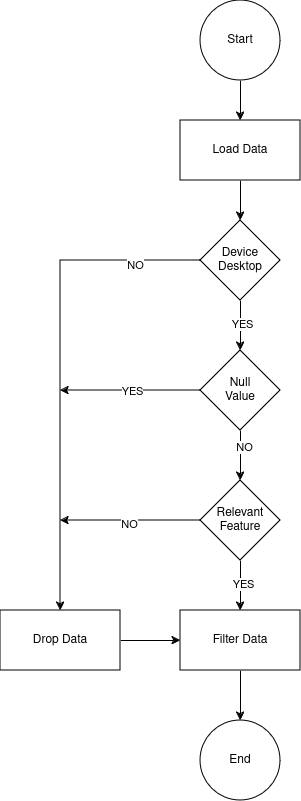
\includegraphics[width=0.4\textwidth]{BAB_TESIS/IMAGES/pre_processing.drawio.png}
    \caption{Rancangan Pembersihan Data}
    \label{fig:pembersihan-data}
\end{figure}

Dalam melakukan pembersihan data, sistem ini akan dua metode yaitu :

\begin{enumerate}
    \item \textit{Missing Value} : Menghapus data yang memiliki nilai kosong.
    \item \textit{Duplicate Elimination} : Menghapus duplikasi data sehingga hanya satu dari data duplikat yang disimpan. 
\end{enumerate}

Pembersihan tahap satu dapat dilakukkan menggunakan fitur pandas yaitu isnull. Setelah itu didapatkan jumlahnya dengan sum. Dengan cara ini didapatkan jumlah data kosong untuk setiap fitur. Untuk fitur yang terdapat nilai kosong akan dibuang
Pembersihan tahap dua dilakukkan dengan cara menyaring fitur \textit{User Agent and Device Type} 
Setelah data dibersihkan, data akan digunakan sebagai input untuk melakukan analisis risiko autentikasi. Data ini kemudian akan digunakan sebagai input untuk melakukan analisis risiko autentikasi.
